\chapter{仿真系统实验设计}
本方案是将原始数据块的哈希信息等密钥相关的数据存放在单独的固态盘上,要求这种固态盘內建的TRIM和安全删除命令已经被厂商正确地实现,而加密后的数据是存放在以固态盘组成的阵列上的,每个加密数据单元存储在阵列的一个条带上,写入数据的时候按照方案设计的缓存模块,依次顺序写到每个条带上,读取的时候,由于输入缓存支持并行传输,利用了阵列并发IO的特点,快速读取到缓存中并且按序存放。要使得原始数据无法再被恢复,擦除掉密钥盘上的哈希信息,或者破坏方法预设的条带数量临界值的数据,就可以达到数据安全的结果。


采用本方案可以实现多种原型系统,例如,基于iSCSI平台,原始数据经过方案实现的系统加密,产生的加密数据分发到以TCP/IP相互连通组成的阵列上,解密数据时只要通过网络读取到各个存储点上的加密数据以及存储在单个盘上的哈希信息,完成解密操作即可。


为了方便验证方案,实验选择了环境相近的仿真实现。仿真实验环境也要求有一个单独的闪存盘用以存储加密的哈希信息参数数据,并且这个固态盘能够做到数据的安全删除,以及TRIM命令的內建实现,为了容易实现,是在以固态盘组成的阵列上划分分区,成为一个个独立的存储单元来存放加密之后的数据单元这种设计,来完成仿真实验。
\section{实验目的}
采用仿真实验主要有以下三个方面的目的:
\begin{itemize}
	\item 确认方案能够达到盘阵数据安全删除的要求。具有可行性。
	\item 仿真测试不同安全级别下,方案在带宽、I/O时延、系统负载、数据冗余率等维度的性能表现,验证方案是否可靠。
	\item 通过较容易实现的仿真环境来进行测试,确保方案针对所有固态盘阵都具有可用性。
\end{itemize}
\section{实验环境}
仿真实验环境硬件配置如\autoref{tab:2}所示。
\begin{table}[H]
    \centering
    \caption{实验环境硬件配置}
    \label{tab:2}
    \begin{tabular}{|c|c|c|}
        \hline
        类别 & 型号 & 数量 \\ \hline
        CPU & Intel(R) Xeon(R) L5520  @ 2.27GHz & 16 \\ \hline
        内存 & 16GB & 1 \\ \hline
        密钥盘 & SV300S37A 120G & 1 \\ \hline
        数据盘 & SV300S37A 120G & 4 \\ \hline
    \end{tabular}
\end{table}
\section{实验方案}
本次仿真实验使用了4块SSD组成的阵列,然后分为4个独立存储区域作为冗余加密数据的存放点。一块单SSD盘作为密钥存储盘。数据块信息虽加密块信息分散存储在数据盘阵上。整体测试流程如\autoref{fig:15}所示。
\begin{figure}[H]
	\centering
	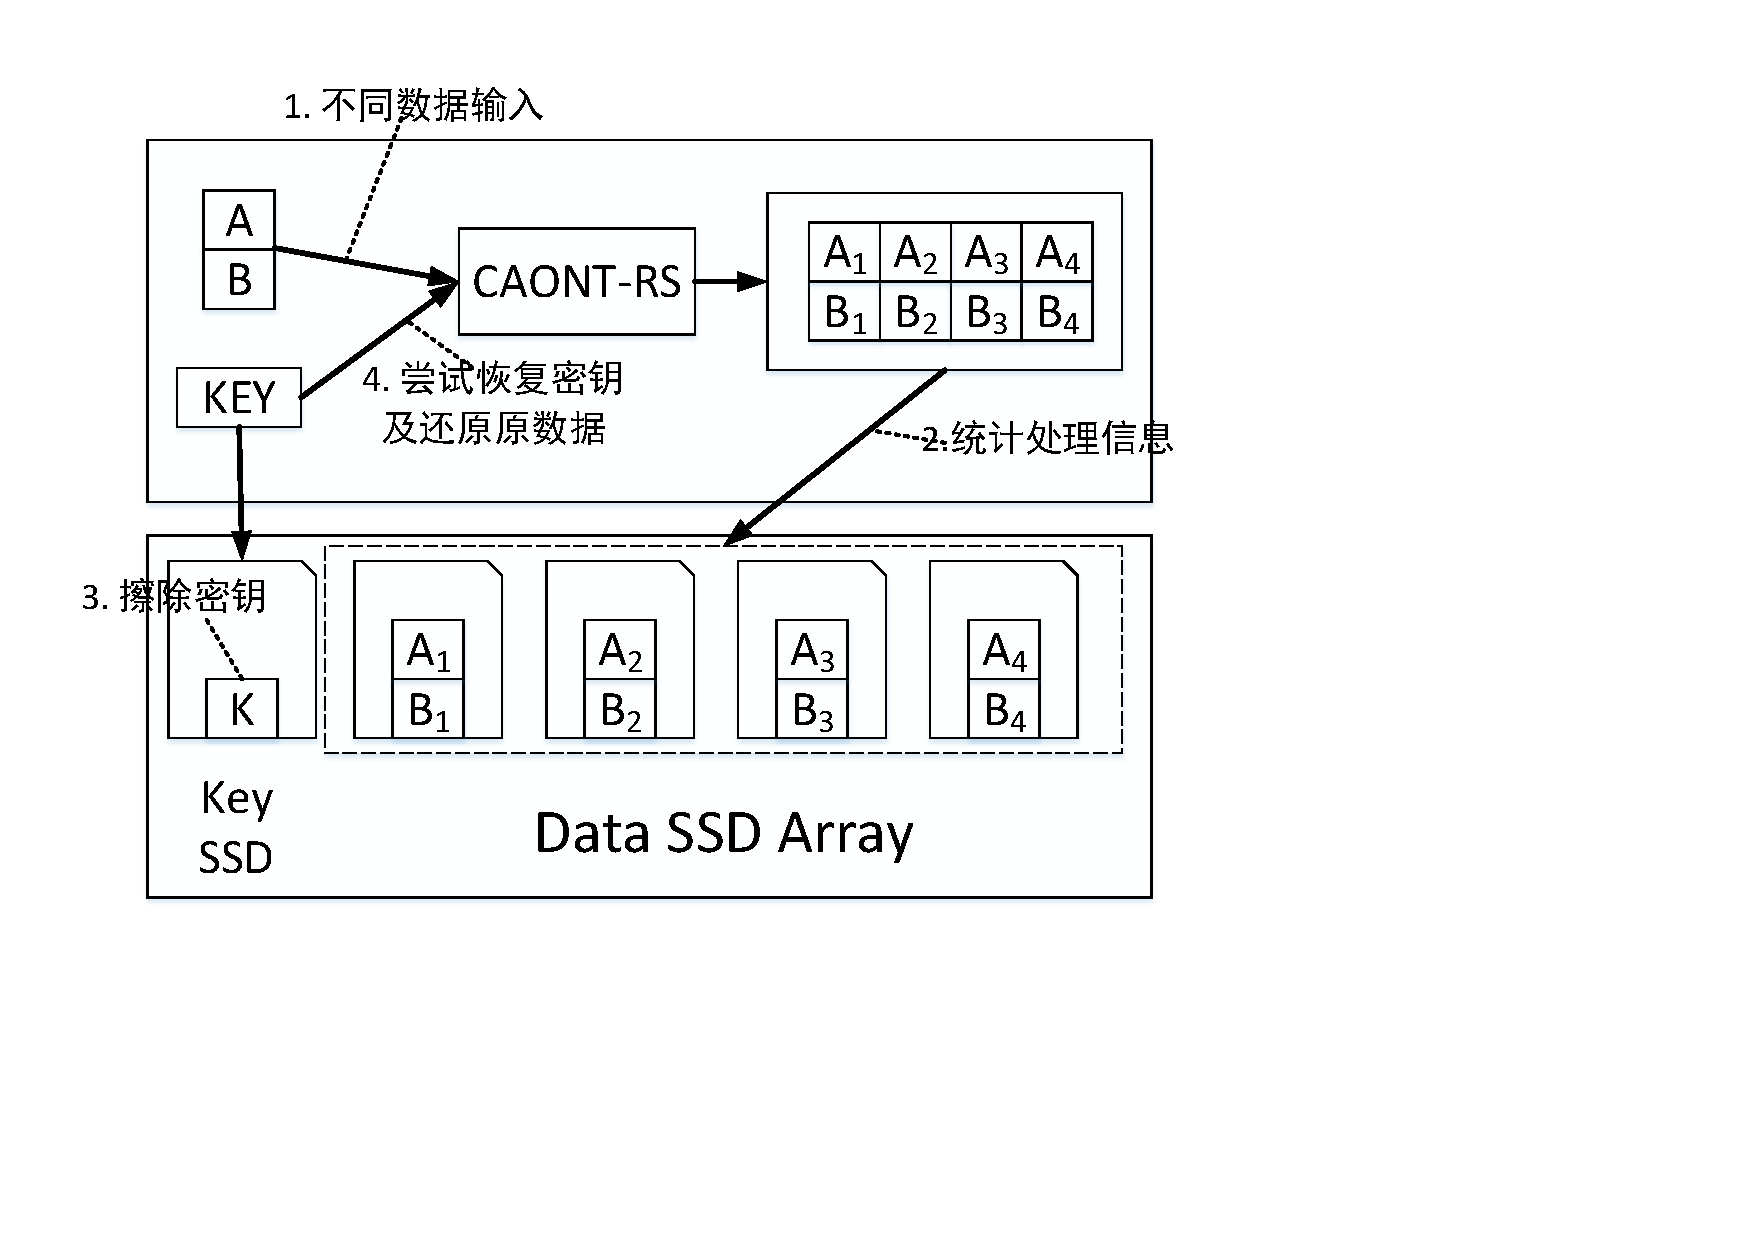
\includegraphics[width=4in]{Pics/test-pr.pdf}
	\caption{测试流程}
	\label{fig:15}
\end{figure}
\begin{enumerate}
	\item 从1MB到1024MB大小的原始数据依次输入仿真系统中
	\item 记录数据从读取到第一块数据被冗余加密,分发到阵列的过程中每个环节所消耗的时间,生成数据的大小以及系统运行状态等相关数据
	\item 记录加密数据读取到被加密模块解密,最终还原为原始数据的各个环节的时间、状态等数据
	\item 使用经过验证的安全删除软件将存储的密钥盘的哈希信息等数据擦除,尝试还原数据,验证安全删除功能
	\item 统计仿真系统测试数据,得到功能测试和性能测试等结果
\end{enumerate}
仿真环境结构如\autoref{fig:16}所示。
\begin{figure}[htb]
	\centering
	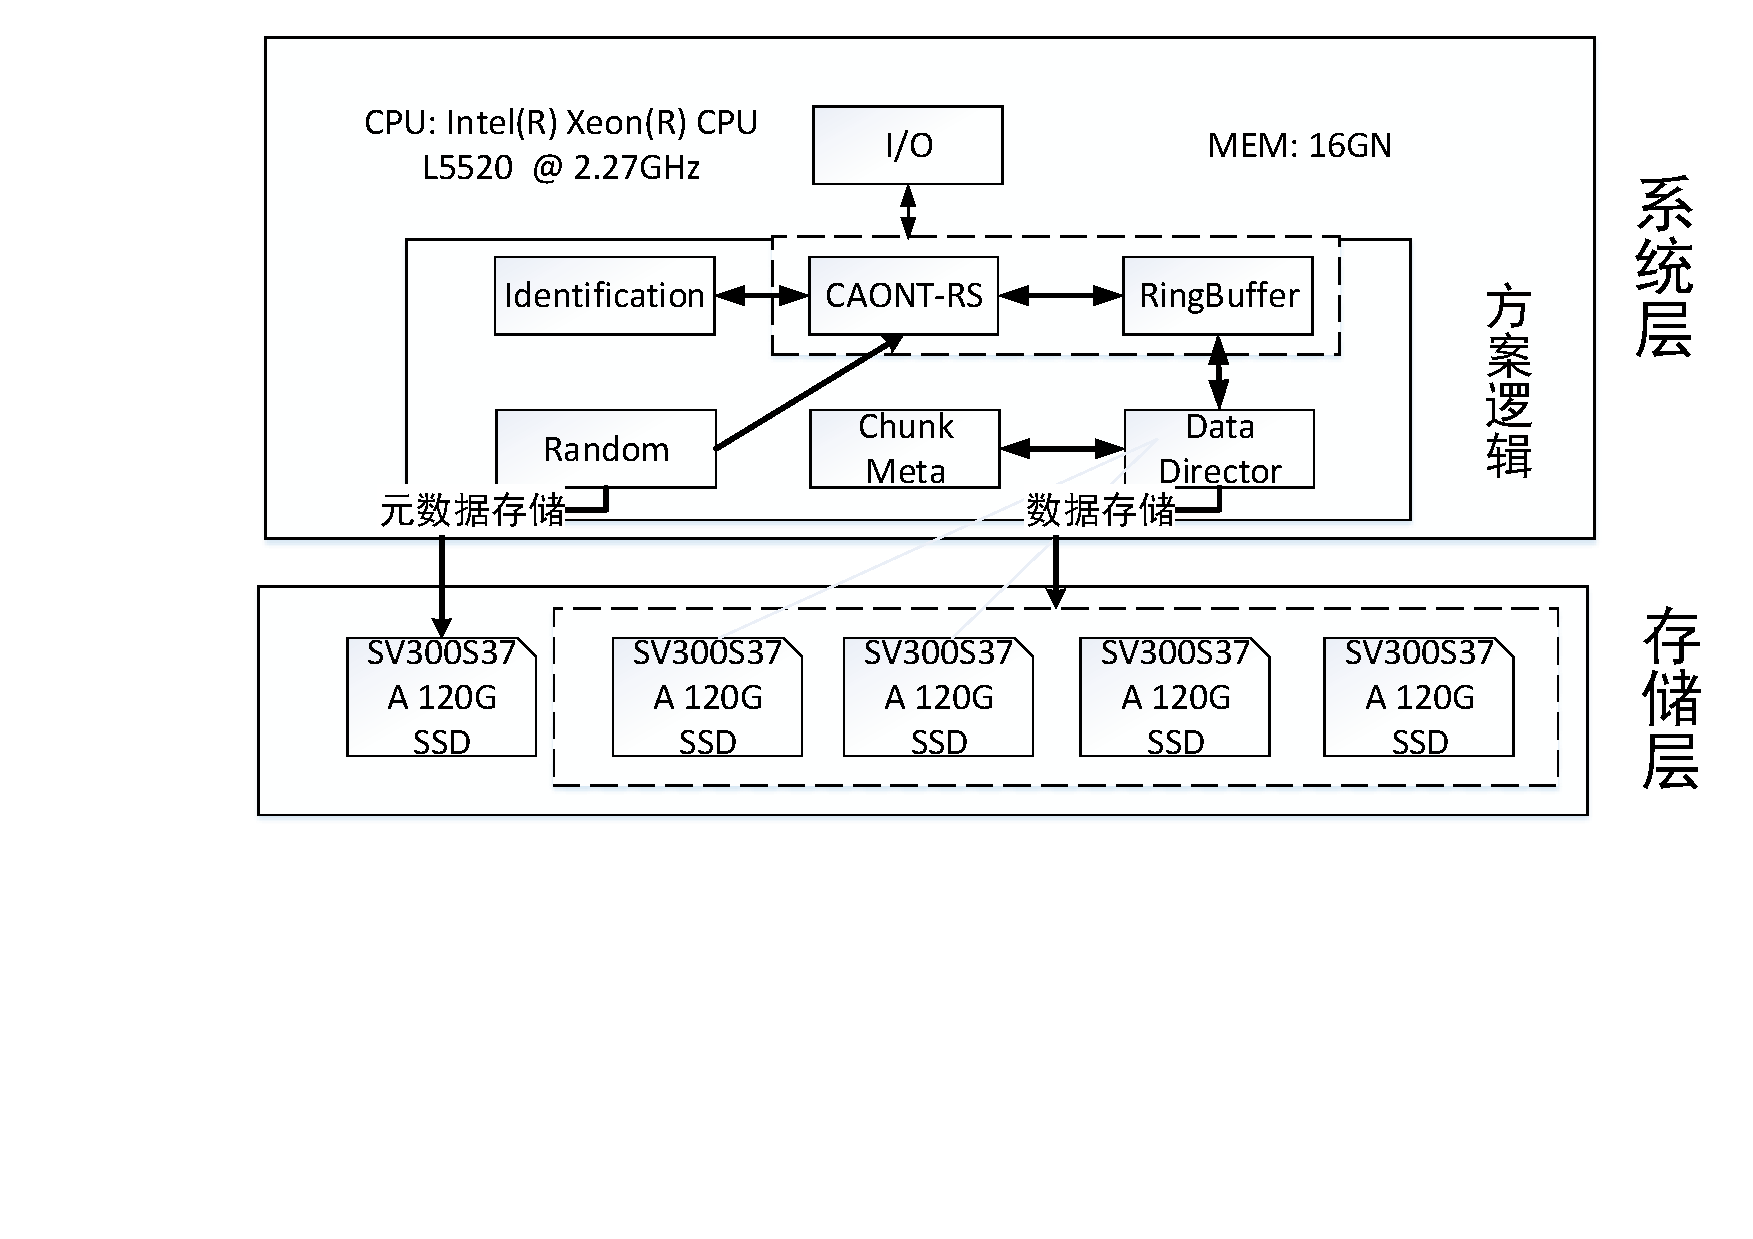
\includegraphics[width=1\textwidth]{Pics/test-env.pdf}
	\caption{仿真环境系统图}
	\label{fig:16}
\end{figure}
\section{仿真系统实现}
\subsection{数据结构设计}
数据结果部分,编码和解码的逻辑处理单元都有两个分别处理输入和输出的数据缓存中心,而这两个缓存中心得数据结构都是以线程安全的循环队列为中心,因此,设计一个多线程高效的循环队列成为了提高数据缓存效率的关键。\autoref{fig:17}和\autoref{fig:18}分别代表了编码输入缓存和输出缓存。
\begin{figure}[H]
	\centering
	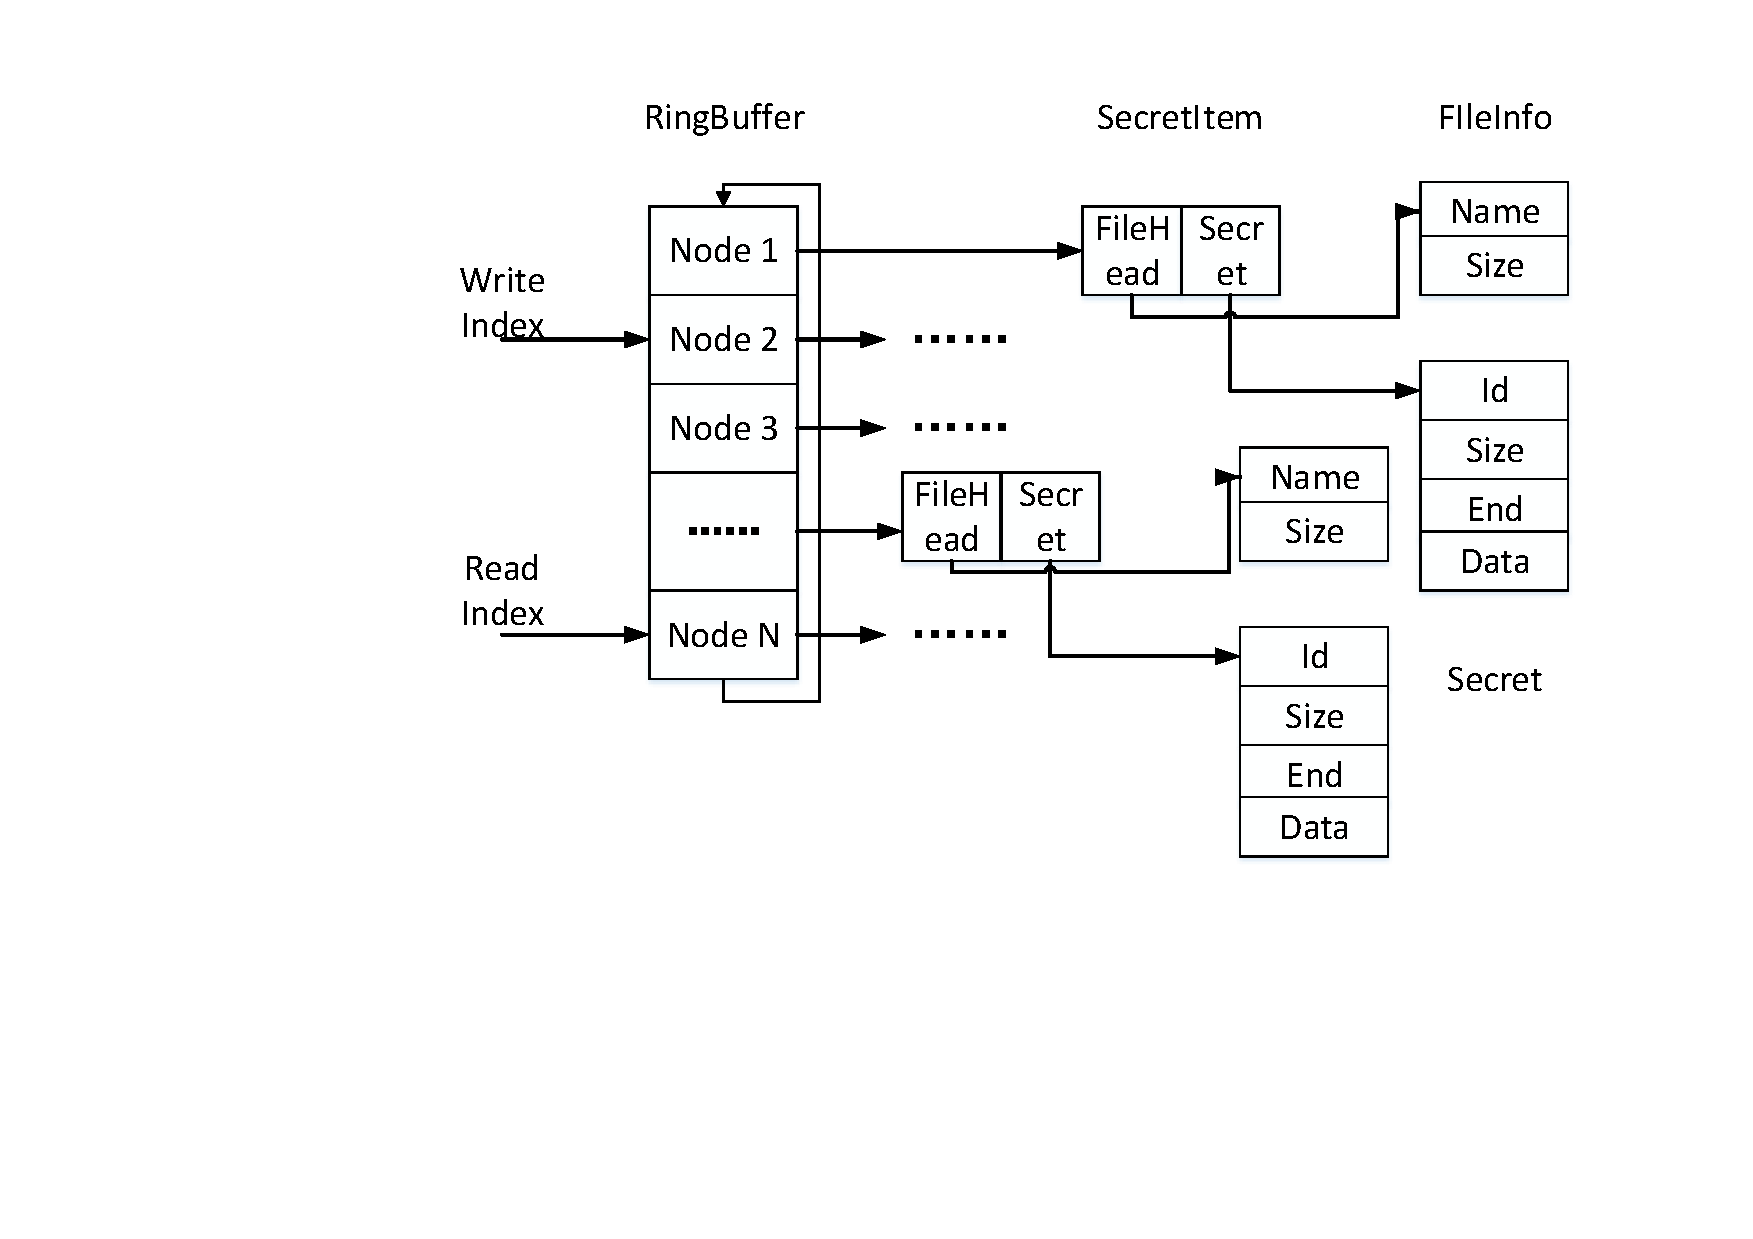
\includegraphics[width=1\textwidth]{Pics/input-buf.pdf}
	\caption{输入缓存数据结构设计}
	\label{fig:17}
\end{figure}
\begin{figure}[H]
	\centering
	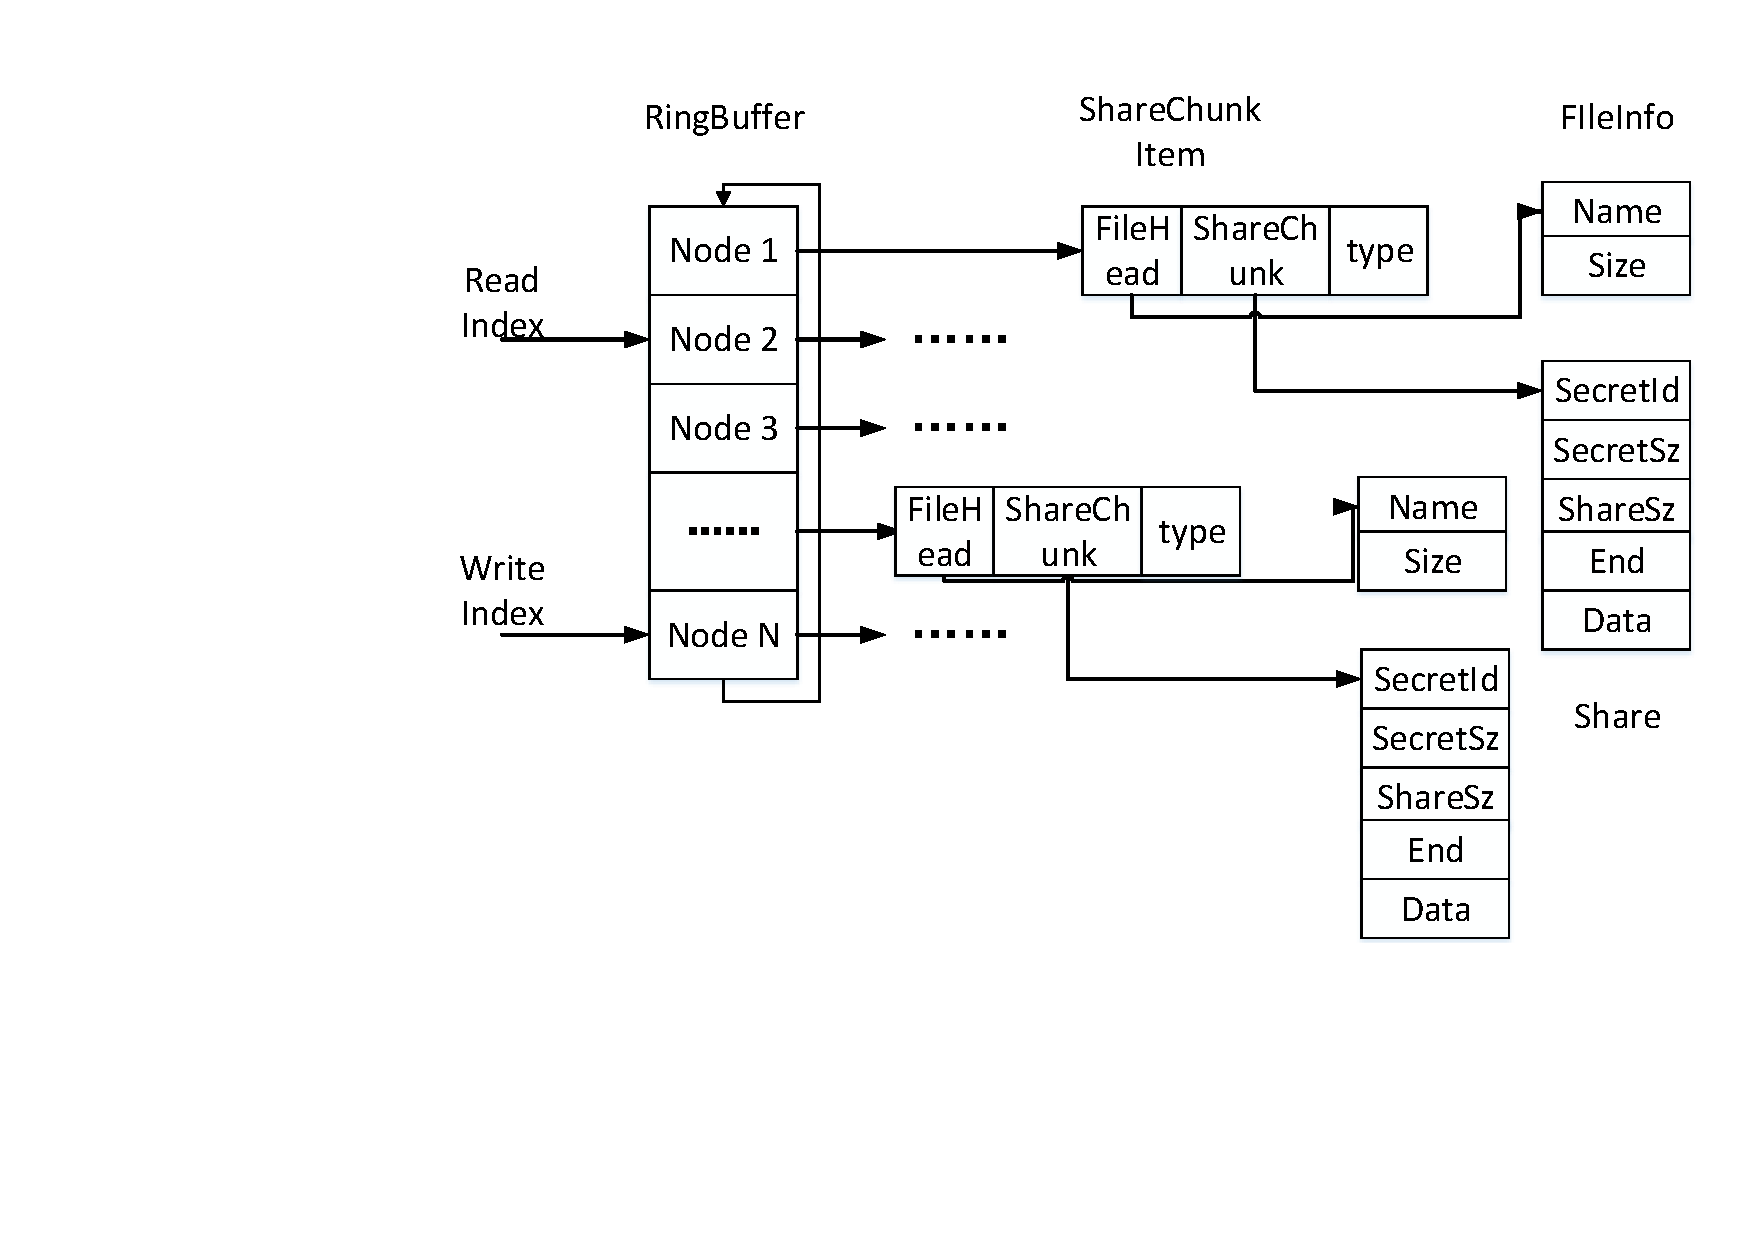
\includegraphics[width=1\textwidth]{Pics/output-buf.pdf}
	\caption{输出缓存数据结构设计}
	\label{fig:18}
\end{figure}
在数据进行编码时,使用如\autoref{fig:17}所示的缓存数据结构,当一个数据块被加密处理完,生成加密数据块后,循环队列在当前写结点开辟一个新的内存,存放原始数据块的文件名、文件大小信息,加密子结点指向一个加密块的序号Id,大小Size,是否是最后一个加密块的标志End,以及最终的加密数据块Data,同时,写索引向后移动一个结点位置,这样一个加密块的缓存过程就结束了。如果写索引后面是读结点,说明队列的缓存已满,队列将在接下来的一段时间拒绝数据缓存请求。


当缓存需要写入到数据盘时,循环队列的读索引获取加密数据块的Id,按照数据盘的个数取模,决定存储在哪个数据盘,队列将当前的读结点的数据传递给数据存储线程,读索引向后移动一个结点位置,缓存读取过程结束,如果读索引后面位置是写结点,则表明当前循环队列已空,接下来的一段时间内数据存储请求将被队列忽略,相关线程也会陷入休眠,知道有数据到达。


加密数据解码时,使用的是如\autoref{fig:18}所示的缓存结构,相关的读写操作刚好和编码相反,只是输出缓存的相关结点内容发生了变化,首先是队列的结点指向的是一个原始文件信息和加密数据块联合的结构体,由类型标明这是一个数据块还是信息块,其中数据块部分相比编码前是多了一个表示最终的冗余加密数据块的大小。数据块依然是由标记End标明是否是最后一个数据块,在数据解密流程起到通知模块解密结束的作用。
\subsection{关键流程实现}
%在方案设计的数据处理流程中,主要做了以下几个比较具体的实现和改进。
\subsubsection{将数据读写模式进行了改进优化}
为了提高系统处理数据的整体性能,除了设计一种比较高效的循环队列以外,方案还对数据存取的具体环节进行了优化设计。以实验系统中的四个数据盘来说,在编码过程中,编码器会将编码完成的数据按照其编号顺序依次存入各个盘对应的循环队列中,各个队列之间的数据缓存以及写入是相互独立的,这样带来的好处就是,相比一个循环队列,数据缓存和存储的数据同步冲突更小,线程切换的次数减少,从而可以并行地存储数据到各个数据盘。


同时在解码时,由于编码算法的特性,只需要读取k份数据即可将原始数据还原出来,具体到本方案中,相比编码需要传输四份数据单元,解码的时候只要读取其中任意三份数据,有效的节省了数据传输的带宽,也减少了等待数据缓存的时间,系统处理性能自然就提升上去了。整体流程架构如\autoref{fig:19}所示。
\begin{figure}
	\centering
	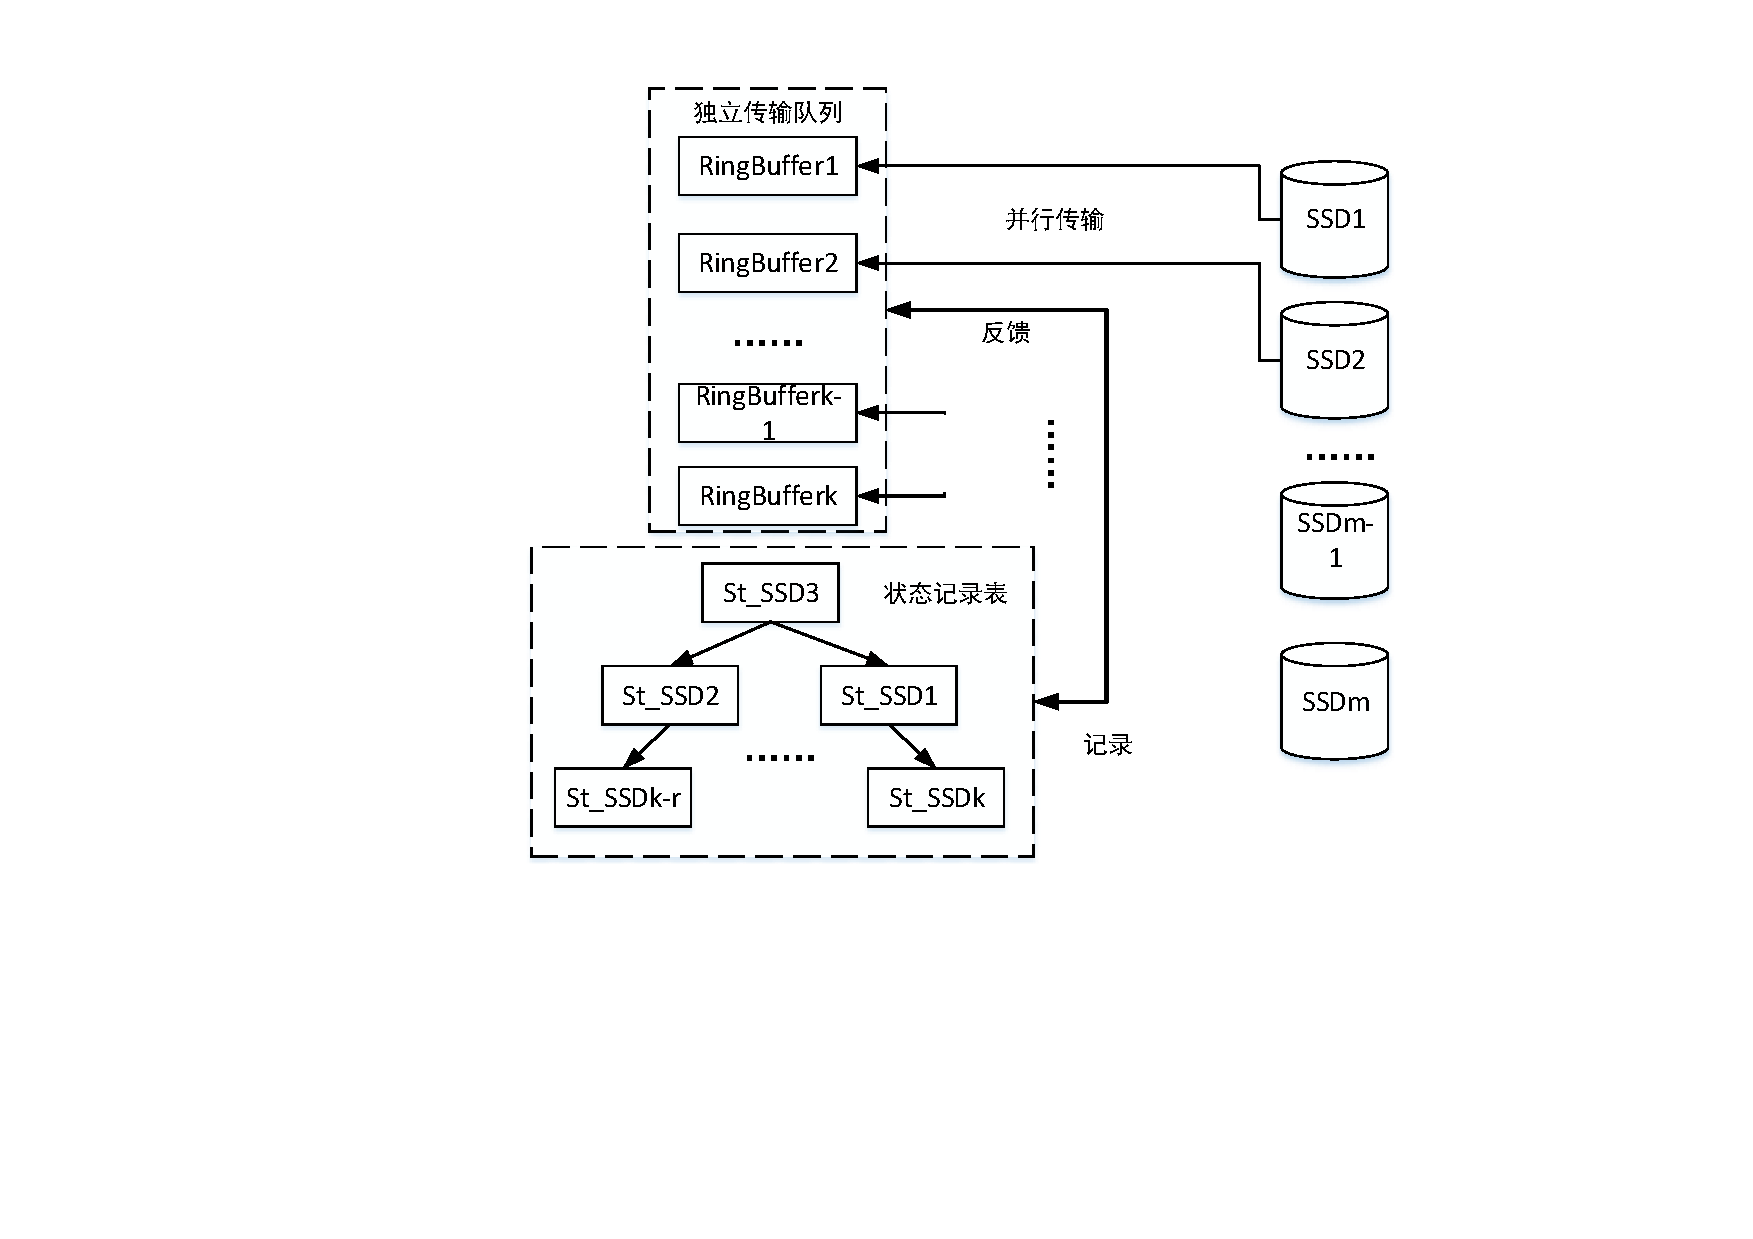
\includegraphics[width=1\textwidth]{Pics/parallel-read.pdf}
	\caption{输出缓存架构设计}
	\label{fig:19}
\end{figure}
另外一个改进是,每次传输数据时,系统都会记录下当前各个数据盘的状态,依据这个状态在那些综合性能比较好的数据盘上优先读取数据,这样带来的一个好处是,系统的容错性大大提升。以测试的4个盘为例,假使有1个盘损坏,也不影响数据读取还原,在比测试规模大很多的环境下,因为数据盘的损坏可能性比较明显,这种容错性带来的优势更加明显,数据的完整性也得到了保证。同时,系统选择那些性能较好的数据盘读取数据,也有效地避免了因为单盘影响其他所有数据盘读取性能的问题。
\subsubsection{实现了密钥数据存储到密钥盘的策略}
由于环境、操作系统等问题造成的不可抗力,都可能使得这套系统崩溃,由于初始密钥向量是随机化生成的,此时仍在内存中,就会因为系统崩溃而丢失,原始的数据无法再通过系统解密再恢复出来,造成了数据丢失。现有的设计对这一问题的解决方法是,在每次处理完数据加密后,密钥模块负责将本次生成的密钥数据存储到单独的密钥盘,设计的密钥存储结构如\autoref{fig:20}所示。
\begin{figure}[H]
	\centering
	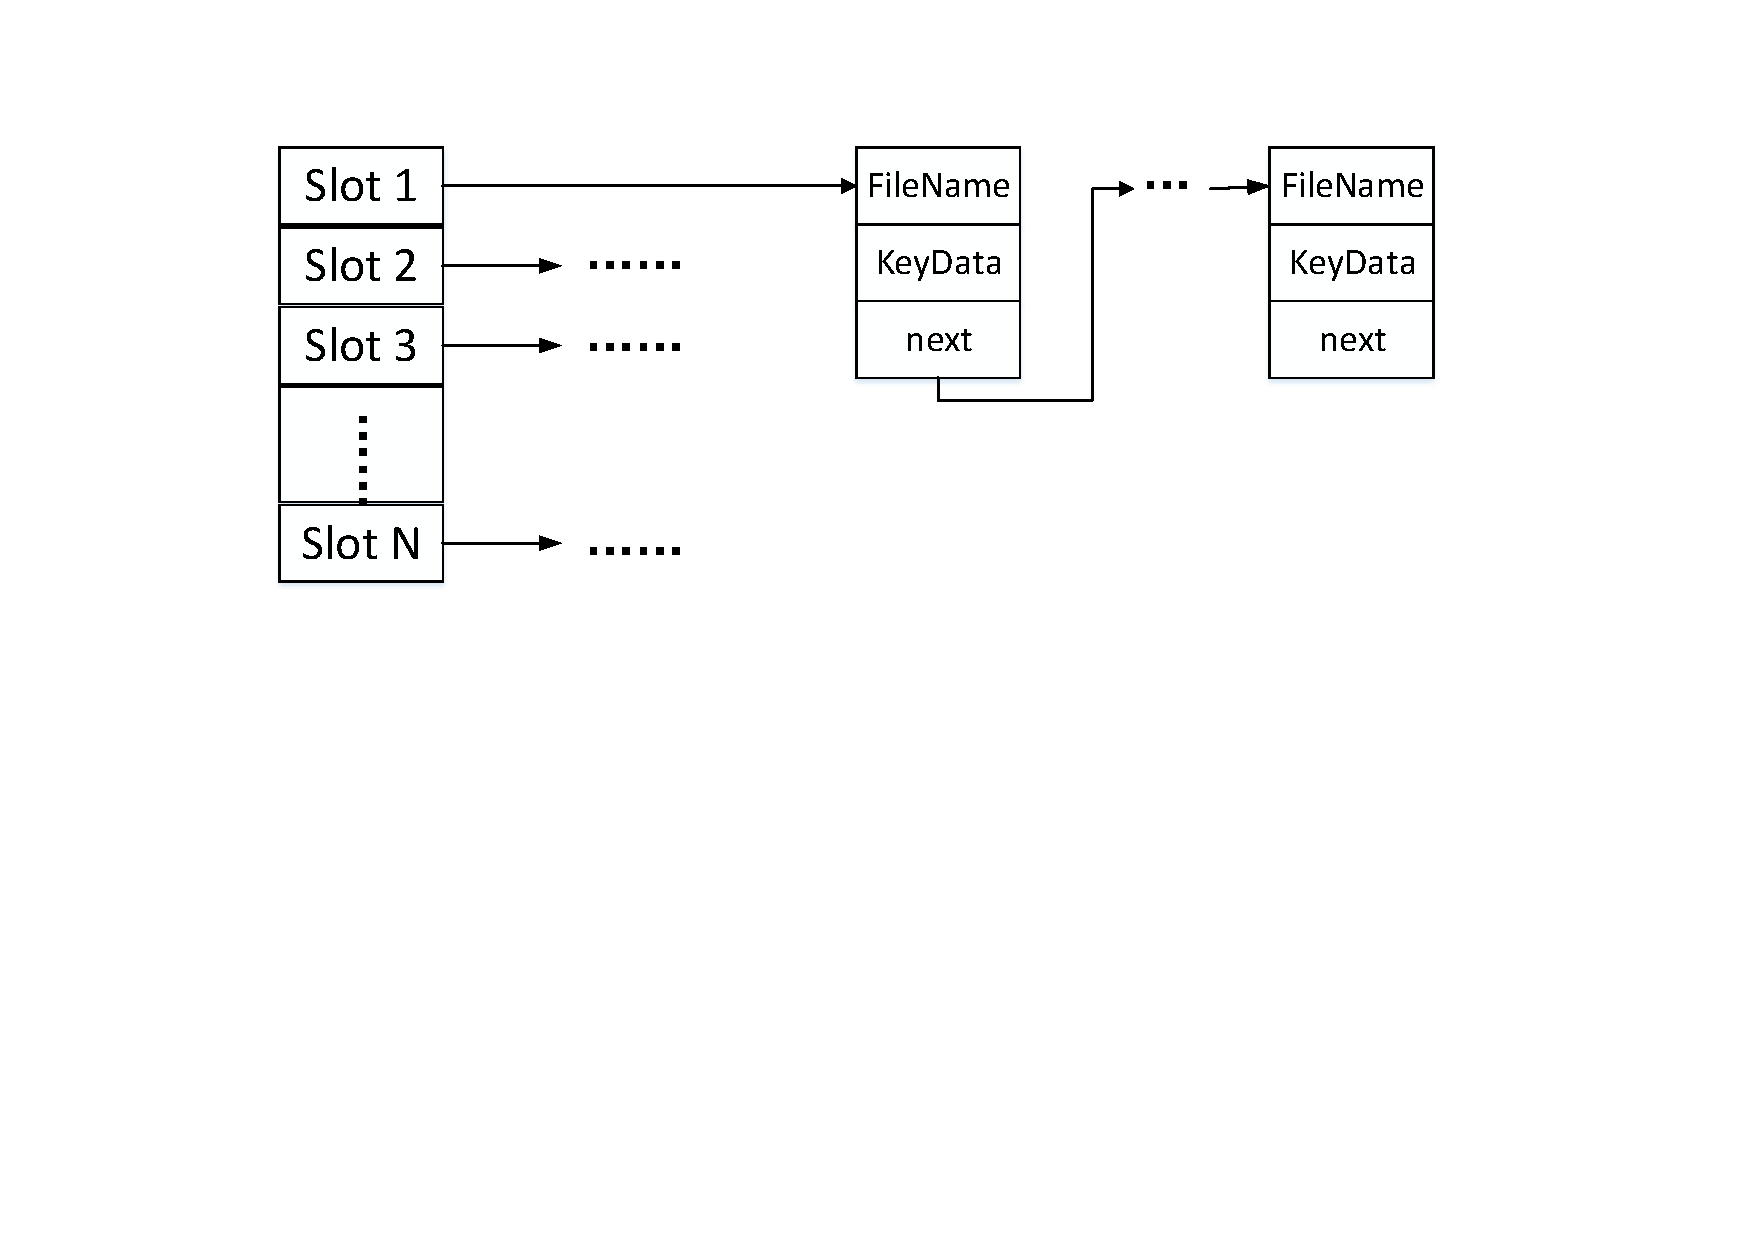
\includegraphics[width=1\textwidth]{Pics/keystore.pdf}
	\caption{密钥存储结构}
	\label{fig:20}
\end{figure}
这样,在系统重启后,对于存储过的文件信息,系统会优先在密钥盘中查找密钥信息,如果是读取还原数据,直接使用密钥信息即可,对于重新存储请求,只需要覆盖掉原来得记录即可。
\subsubsection{加密算法实现}
 \begin{algorithm}[H]
 	\caption{Encode origin data with hash info.}
 	\label{alg:2}
 	\begin{algorithmic}
 		\REQUIRE $secret buffer,m \ge k$
 		\STATE $B \gets bytesof per secret word$
 		\STATE $S \gets secret buffer size$
 		\STATE $A \gets aligned secret buffer size$
 		\ENSURE $A \le min\{(S+B) \% (B+K), B*(k-1) / (B*k+1)\}$ 
 		\STATE $shareSize \gets (A / B + 1) / k * B$
 		\STATE $aligned buffer \gets secret buffer$
 		\STATE $Key \gets Generate Hash with aligned buffer$.
 		\FOR{i = 0 to A}
 		\STATE $aligned size constant Array_i \gets i\&0xff$;
 		\ENDFOR
 		\STATE erasure coding data $\gets$ Encrypt with aligned size constant Array and hash info.
 		\STATE erasure coding data $\gets$ Galois Group multiply region hash info with value 1 and,step by B,adding by 1.
 		\STATE share buffer $\gets$ erasure coding data
 		\FOR{i=0 to m}
 		\FOR{j=0 to k}
 		\STATE $value \gets distribution_{k^2+k*i+j}$;
 		\STATE
 		share buffer $chunk_{k+i} \gets$ Galois Group multiply region,
 		share buffer $chunk_j$ with value ,
 		step by shareSize,adding by 1 $if j \neq 0 else 0$
 		\ENDFOR
 		\ENDFOR
 		\RETURN share buffer
 	\end{algorithmic}
 \end{algorithm}
加密算法\autoref{alg:2}中,关键的操作主要有,首先根据对齐的原始数据块生成它的哈希值,作为该数据块加密的密钥,使用常向量constant array加密并且群运算之后得到初始的加密数据块,之后就按照每个冗余数据单元的大小从前往后依次群运算得到每个加密的数据块,后面的加密单元依赖前面已生成的加密单元。
\subsubsection{解密算法实现}
\begin{algorithm}[H]
	\caption{Decode encrypted data with Key(hash info)}
	\label{alg:3}
	\begin{algorithmic}
		\REQUIRE{share buffer,kShareID,k}
		\STATE B $\gets$ bytesof per secret word
		\STATE S $\gets$ secret buffer size
		\STATE A $\gets$ aligned secret buffer size
		\ENSURE {shareSize \% B = 0 $\vee$ erasure codeing data size $\ge shareSize * k$}
		\FOR{i=0 to k}
		\FOR{j=0 to k}
		\STATE $squared matrix_{k*i+j} \gets distribution_{k*kShareID_{i}+j}$
		\ENDFOR
		\ENDFOR
		\STATE invert squared matrix
		\FOR{i=0 to k}
		\FOR{j=0 to k}
		\STATE value $\gets squared matrix_{k^2+k*i+j}$;
		\STATE erasure coding data $chunk_i \gets$ Galois Group multiply region  share buffer $chunk_j$ with value ,
		step by shareSize,adding by 1 $if j \neq 0 else 0$.
		\ENDFOR
		\ENDFOR
		\STATE Key $\gets$ Generate Hash with erasure coding data.
		\STATE Key $\gets$ Galois Group multiply region  erasure coding data with 1 ,step by B,adding by 1.
		\STATE erasure coding data $\gets$ Encrypt with aligned size constant Array and hash info.
		\STATE aligned sercet buffer $\gets$ Galois Group multiply region  erasure coding data with 1 ,step by aligned secret size,adding by 1.
		\STATE erasure coding data $\gets$ Generate Hash with aligned sercet buffer.
		\STATE secret buffer $\gets$ aligned sercet buffer
		\RETURN secret buffer
	\end{algorithmic}
\end{algorithm}
解密算法\autoref{alg:3}中,首先根据分散向量和当前的冗余数据单元运算得到解密矩阵squad matrix,然后逆置,并作为接下来的群运算的乘积因子,从冗余数据单元的每个数据块从前往后依次得到相应的初始加密数据,初始加密数据的末尾信息部分在群运算和解密操作后得到原始数据块的哈希值,使用该哈希值与初始加密数据再次群运算和取哈希操作,就得到了最终的原始数据块。
\section{本章小结}
本章阐述了依据全闪存盘阵数据安全删除的原型系统实现的仿真系统。
主要分为四个部分,首先介绍了采用仿真实验的目的和仿真环境的系统结构,其次列出了仿真实验的大体步骤,
最后详细描述了仿真系统中的数据结构设计和关键流程实现,总结出系统的存储哈希信息等数据到单独的密钥盘,
以及加解密算法设计的实现。
